\chapter{Concept and Design}
\label{cha:conceptanddesign}

This section is a theoretical introduction to the modules required for macroscopic movements modeling and visualization. There are three main modules in this project which can work independently from each other:

\begin{itemize}  
\item Stop location detection
\item Clustering of detected stops 
\item City Movements Graph and Analysis
\end{itemize}

\section{Type of data available}

The data supplied to the system is based on tracking and geofencing proactive location-based
service, targeted at end users and retailing companies, as discussed in \autoref{cha:introduction_hummob}. The accuracy of user location is biased not only on accuracy of position estimation used by mobile device, but also by the technological and commercial limitations of the data acquisition strategy of geofences. This means that data is spatially sparse, coarse and its resolution depends on density of geofences.
\\\\
Thus, recorded data points are associated with unique user id, timestamp, latitute and longitude of the position at which user have been found to move from one area to another.

\begin{figure}[!ht]
	\centering
	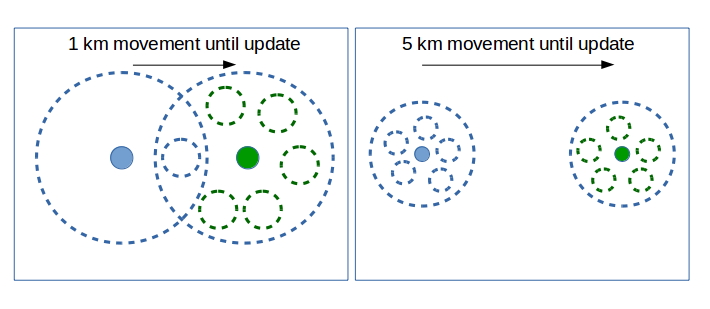
\includegraphics[width=0.9\textwidth]{images/movement_update.png}\\
	\caption{Continuous and Discontinuous location update after movement to section lacking area details }
	\label{fig:movement_update}
\end{figure}
\FloatBarrier

Because of the characteristics of GPS and other positioning methods, in so called urban street canyons and the like, signal loss with re–acquisition times of 45 seconds to five minutes can be observed \cite{StopDet1}. This could lead to discontinuous recording of the location - \autoref{fig:movement_update}.

Another aspect to consider is the fact that because of commercial application of the available data might be targeted to a specific user group, the macroscopic movements analysis might not be representative for the population in general (for example, position data  collected from a running application would probably generate different points the one for finding restaurants).

\section{Stop location detection}

In the context of macroscopic movements of people, stop detection is required to identify, based on supplied data source, whether the person under observation has stopped, at what location and how long he stayed at that location. The challenge for stop detection, in the context of proactive location-based services, is the method of data collection. Firstly, each location is recorded due to movement from one area to another. This means, that person might have stopped somewhere in between these points, and stop detection should be able to identify both location and duration of stay. Furthermore, if a user enters an urban canyon, building or move underground, the signal might need to be re-obtained after a movement to new area. This loss of signal can take some time, where points possibly can be spanned over mid-range/long distances. On the other hand, points received over a short distance might mean that a person has been already been moving with a good signal reception .

\subsection{Mobility index based approach}
\label{cha:stopdet_mi}

We decided to reuse the concept of mobility index, having artificially created areas in the city. In this case, the location point is recorded whenever moving into a new geographical area and requesting an update.
\\\\
In a populated area, the user can move from one area to another, and the movement can take from seconds to several minutes. Thus, if within a certain
period of time (called mobility index time window) the user stays in the same area or changes the areas with small pace (mobility index is below certain threshold) it can be assumed that the user is immobile or approaching stop location and having a stay somewhere within that time window (restricted area). 
\\\\
There are two approaches to calculate mobility index - having equally spaced windows in time, or sliding window.

\begin{figure}
	\centering
	\begin{minipage}{.45\textwidth}
		\centering
		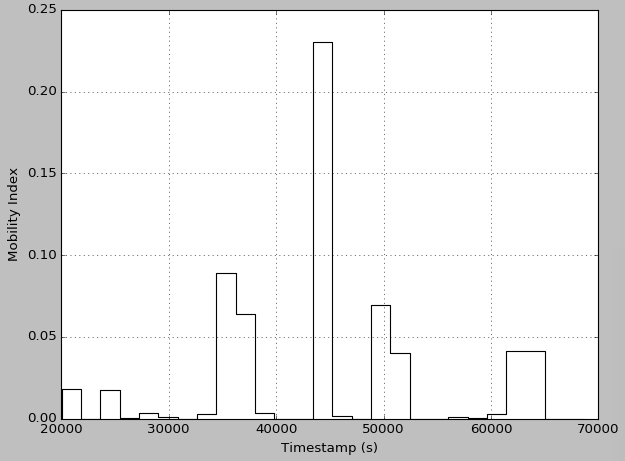
\includegraphics[width=.9\linewidth]{images/mob_calc1.png}
	\end{minipage}%
	\begin{minipage}{.45\textwidth}
		\centering
		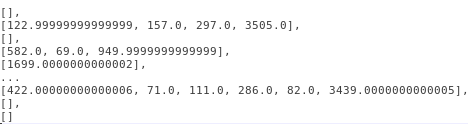
\includegraphics[width=.9\linewidth]{images/mob_calc2.png}
	\end{minipage}
	\captionof{figure}{Mobility Index calculation using equally spaced windows in time (left) and using sliding window over time (right). Time Window of 30 minutes using the same data set for one unique user}
	\label{fig:mob_calc}
\end{figure}

\FloatBarrier

In the first approach, for a single user, minimum and maximum timestamp of sorted sequence is found. The function is creating equally spaced bins of that value within the maximum and minimum timestamps. Each point is visited and assigned to the proper timestamp-bin according to its timestamp and duration to the previous point. 
The disadvantage of this approach is that points and their duration are randomly placed in bins, which could lead to representing mobility of fixed window, instead of mobility history for points.  
\\\\
In the second approach each point of a user is being visited and temporarily marked as "current position". For each current position, all points which are distant in time by the mobility index window in the past are assigned to the sliding window. The advantage of this approach is that it precisely represents the mobility history in the past duration window.

\subsection{Human Behavior based approach}
\label{cha:stopdet_bh}

This section describes the approach and conditions for movement between two points that has to be satisfied in order for the point to be a considered a stay. 
\\\\
The \autoref{cha:introduction_hummob} discusses, that in average, a walking human is traveling with the speed of over 3km/h up to 5km/h. However for movement over long distances, a user will most likely use a city or private transport, thus her speed might vary drastically in that time/distance period.
\\\\
This approach states, that if movement between two points has been recorded within short distance, and movement of speed is below a certain threshold, it might mean that user has stopped or has been moving very slowly within a restricted area. This is called a \textbf{possible stop} for that location between these points. 
\\\\
For movements between points over mid/long distances recorded, a user might have stopped at the first location, moved with different speeds between points and then continued moving (proactive localization is used). As an example, movement over 6km might require up to 10 minutes with transportation. If the user stopped at previous location for 20 minutes, the total movement between point took 30 minutes, which in average is about 12 km/h. Universal speed threshold is not able to detect stops in these kind of examples, since travels over higher speeds with stop at previous location would result in relatively high average speed. 

\section{Clustering of stops}

After our stop detection algorithm has detected the proper stops we need to analyze them. Our goal is to retrieve the overall movement patterns of a population within a certain area, which means we are interested in \textbf{macroscopic} movements and not microscopic (individual) movement. If we would consider every individual our analysis algorithms would get fed with a lot of noise (outliers) which would make data mining and prediction difficult and inaccurate. Meaning, \textit{Macroscopic Movements} are not interesting in tracking individuals but rather seeing the big picture.

 Once the clustering algorithm has been applied and we have the overall picture, we can see which stops are most popular, where people are moving from them, and how long they stay at a certain location. One could then perform some interesting graph analysis on these locations, answering questions such as "what is the probability that a person moves from point \textit{A} to \textit{B}?", or "what is the average stop time at location \textit{A}?". 
 
 To achieve these clusters, which represents our interesting stop locations, we need to apply some clustering algorithm. DBSCAN, described in \autoref{cha:relatedwork}, was our approach of achieving these clusters.  

\FloatBarrier
\section{City movements graph}
\label{cha:movementsGraph}
This section introduces the concepts and terms related to graph analysis used in this project. Our target is to identify popular locations and routes in a city and determine movement patterns of people. The stop points identified by the stop algorithm correspond to actual physical locations in the city with individual latitude and longitude values. These stop points are clustered to identify places of interest in the city. A collection of such stop clusters can be used to chart the movement patterns of the residents.

\subsection{Basic concepts}\label{cha:basicConceptsGraph}The first step of creating a user movement graph is to create vertices and edges.It is important to outline how the vertices and edges have been selected for creating the city graph. \linebreak
\textbf{Vertices:}Clusters generated by the DBSCAN algorithm are considered as vertices. \linebreak
\textbf{Edges:}For our analysis we are using an edge to represent the trajectory of movement. A trajectory or simple edge is created by joining successive points from individual user movement data.
\linebreak
\textbf{Graph:}The edge set has been used to create a simple directed graph. Direction of movement is considered from the start point going towards the end point or next point in sequence.

An important aspect about our data is that it has been captured over a period of 24 hours. In other words, our user data does not vary over days of a week. In case of such temporal variation of data, day of the week has to be considered while creating the edges.

\subsection{Graphical representation and analysis}
\label{cha:graph1}
 We are using various characteristics of a graph like in- and out-degrees, strongly connected components, betweenness and PageRank \cite{page1999pagerank} for our analysis. We are also using the concept of Origin-Destination Matrix and using the trip counts for modeling the network graph. 
 
 As mentioned in \autoref{cha:graphrelatedworks} , OD matrix is widely used in mobility data analysis and can be used to predict movement patters, important routes etc. From incidence relation between an edge and a vertex, we can calculate degrees(in and out degrees), and can identify hotspots in a city. For example: the central train station or airport of a city will have a high in and out-degree, due to high number of people traveling to and from that place.

 We will be analyzing our directed graph for strongly connected components, betweenness and PageRank. Strongly connected component can give us the areas of the city that are highly interconnected. This connection or route can be roads or transportation networks. For our mobility data, PageRank can provide us with a set of vertices that are most influential or highly accessed. Similarly, betweenness can provide us with nodes that are part of many shortest routes and hence influence the routing decisions by users. For a city, these vertices can correspond to transportation hubs, central business or administrative districts, junction or crossover points.

\FloatBarrier
\FloatBarrier